The details of the metrics selected for quantitative evaluations and that these metrics will be applied on codebases using the CodeMR static code analysis tool are mentioned in section \ref{section:3.2}. However, the information that would facilitate the interpretation of the charts and reports produced by CodeMR was not shared. It is deemed appropriate to share this information in this section so that the results can be understood and interpreted more easily.

The CodeMR tool uses different visualization methods in the reports generated by the application of metrics. The details of these visualization methods and the types of charts used are detailed in the CodeMR documentation \footnote{ \url{https://www.codemr.co.uk/documents/}}. Within this study's scope, the visualization method known as "Metric Distribution" in CodeMR literature and presenting the results in the form of a pie chart was preferred. The main reason for choosing this method is that it makes the visual understanding of the results easier than other methods. Other visualization methods and charts are very detailed, and sharing such detailed results is beyond this study's scope. There are two important points to be aware of when interpreting pie charts created by the "Metric Distribution" method using CodeMR. The first of these points is legends used to indicate metric levels. As can be seeń in Fig. \ref{fig:code-mr-legends}, each colour corresponds to a metric level.
\begin{figure}[ht!]
    \centering
    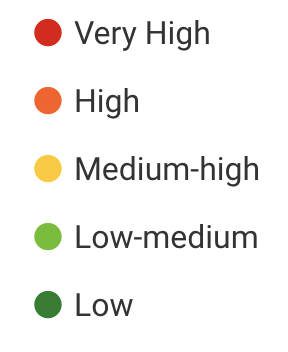
\includegraphics[scale=0.7]{figures/code-mr-legends.png}
    \caption{CodeMR Metric Level Indicators}
    \label{fig:code-mr-legends}
\end{figure}

The second important point is how the percentages on these graphs are calculated while realizing the pie charts created by CodeMR. Below is a pie chart created by CodeMR using the "Metric Distribution" method and the "Size" sample metric.
\begin{figure}[ht!]
    \centering
    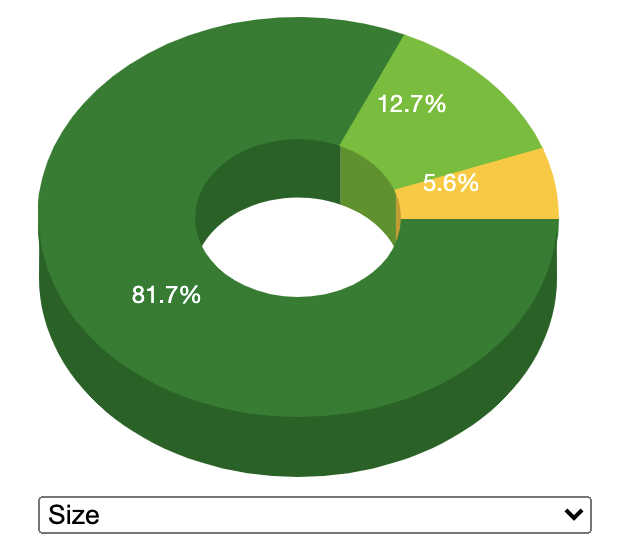
\includegraphics[scale=0.6]{figures/sample-code-mr-chart.png}
    \caption{Sample CodeMR Pie Chart}
    \label{fig:sample-code-mr-chart}
\end{figure}
\FloatBarrier

As can be seen in Fig. \ref{fig:sample-code-mr-chart}, there are 3 different metric levels in different percentages in the graph. These percentages of metric levels for the selected metric are illustrated in a pie chart proportional to the code size of classes in this level. In other words, the slices of pie charts are proportional to the code volume of classes for the corresponding level.

As explained above, these two points are essential when interpreting pie charts that will be shared in the next three sections. In the following sections, the results of this evaluation and the findings for comparisons are shared.

